\documentclass[letterpaper, 12 pt, conference]{ieeeconf}

\IEEEoverridecommandlockouts
% This command is only needed if 
% you want to use the \thanks command

\overrideIEEEmargins
% Needed to meet printer requirements.
%\usepackage[margin=0.65in]{geometry}

% See the \addtolength command later in the file to balance the column lengths
% on the last page of the document

% The following packages can be found on http:\\www.ctan.org
\usepackage{graphics} % for pdf, bitmapped graphics files
\usepackage{epsfig} % for postscript graphics files
\usepackage{mathptmx} % assumes new font selection scheme installed
\usepackage{times} % assumes new font selection scheme installed
\usepackage{amsmath} % assumes amsmath package installed
\usepackage{amssymb}  % assumes amsmath package installed

\usepackage{hyperref}
\usepackage{url}
%\usepackage[pdftex]{graphicx}
%\usepackage{amsfonts}
\usepackage{subfigure} 
\usepackage{algorithm}
%\usepackage{algorithmic}
\usepackage{algcompatible}
\usepackage{framed}
\usepackage{balance}
\graphicspath{{images/}}
\usepackage{multicol}

\title{\LARGE \bf
Generating Natural Language Descriptions of Trajectories Using Long Short Term Memory Neural Networks}

\author{Rodolfo Corona and Rolando Fernandez}

\begin{document}

\maketitle
\thispagestyle{empty}
\pagestyle{empty}

\section{Problem Description}

Given a point-cloud $p$ $\in$ $P$ and a manipulation trajectory $t$ $\in$ $T$, our goal is to output a free-form  Natural Language (NL) description $l$ $\in$ $L$ that describes the trajectory $t$:

\begin{equation}
f: T\times P \mapsto L
\end{equation}

\section{Background on LSTMs}

LSTMs are a variant of the Recurrent Neural Network (RNN) architecture which attempt to alleviate the vanishing gradient problem which traditional RNNs can suffer from. 
\par
LSTMs accomplish this through the use of \textit{gates}, which change the cell's state at each time step based on the current time step's input and the last time step's output. Intuitively, at each time step, an LSTM cell decides which information to forget and which new information to incorporate through the use of its gates. Formally, this computation takes the form of the following gate update equations: 

\begin{align}
f_t &= \sigma (W_fx_t + U_fh_{t-1}+b_f) \\
i_t&=\sigma (W_ix_t + U_ih_{t-1}+b_i) \\
c_t &= tanh (W_cx_t  + U_c h_{t-1}+b_c) \\
o_t &= \sigma (W_o x_t + U_o h_{t-1} + b_o)
\end{align}

And the cell state update and output equations:

\begin{align}
C_t &= f_tC_{t-1}+ i_t c_t \\
h_t&= o_t \cdot tanh(C_t)
\end{align}
Where $\sigma$ is the sigmoid function and, given a gate $g$, $b_g$ is the bias and $W_g$ and $U_g$ are the input and hidden state weight matrices respectively \cite{hochreiter1997long}.  

\section{Methods}

\subsection{Robobarista Dataset}

Sung et al. developed the Robobarista framework in order perform deep multimodal embedding of point clouds and NL descriptions that could be mapped to trajectories, as shown in Equation (8). Sung et al. aimed to create a system for manipulation planning through natural language which could generalize to different objects with similar parts to be manipulated \cite{sung2016robobarista}. 

\begin{equation}
f: P\times L \mapsto T
\end{equation}

Using the Robobarista framework, Sung et al. collected a dataset consisting of triplets of the form $(t, p, l)$. The dataset consists of 116 objects with 249 parts (i.e. 249 point cloud segments) along with 250 NL instructions, for which 1225 manipulation trajectories were collected. 

Each of the 116 objects is split into parts depending on the number of NL instructions that pertain to it and the original point cloud scene is segmented with respect to the part frames, being stored as a Comma Separated Value (CSV) file consisting of [x,y,z,r,g,b] values. 

Furthermore, each of the objects have multiple manipulation trajectories for each part stored as a list of waypoints \cite{sung2016robobarista}. For our experiments, we split the dataset into 5 folds of train and test data in order to perform 5-fold cross validation.

\subsection{Baseline with Point Clouds}
For our initial baseline, we created a pipeline that utilizes the point clouds in the Robobarista dataset to perform inference using K-Means clustering and K-Nearest Neighbors (Figure \ref{fig:Baseline_Point_Cloud}). 

We first train a K-Means model and a KNN model using the training data for each of the 5 folds. The point cloud key points are taken from the segmented object part point cloud CSV files. We create two vectors from the CSV files, one is a vector $\overline{P}$ of all the point clouds in the training set where the point clouds themselves are vectors of key points and the other is a vector $K$ of all the key points in the training set. 

Utilizing the K-Means algorithm in the Python SKLearn package, we cluster the key points in $K$ into 50 clusters and get back a trained K-Means model. With the K-Means model, we extract a cluster prediction for each key point in each individual point cloud in $\overline{P}$. Then, using the cluster predictions as in \cite{csurka2004visual}, we compute a Bag of Features (BOF) vector for each point cloud based on the number of occurrences of each cluster.

The BOF vectors are then used as input with a neighbor count of 1 to the K-Nearest Neighbors classifier in the Python SKLearn package and in return we get a trained KNN model. We are then able to use this KNN model to determine the nearest neighbors of a given point cloud. 


\begin{figure}[htb!]
  \centering
  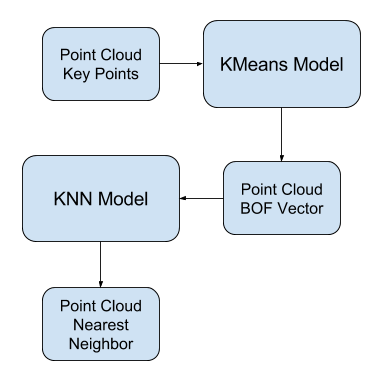
\includegraphics[width=0.3\textwidth]{Baseline-[Point_Cloud]}
  \caption{Baseline model with point clouds}
  \label{fig:Baseline_Point_Cloud}
\end{figure}

\subsection{LSTM Implementation}

We currently implement an encoder-decoder LSTM neural network architecture. Specifically, our architecture uses one LSTM layer to encode the inputted sequence of trajectory waypoints $t$ into an embedding $h$. This embedding is then fed into another LSTM layer which decodes it into a sequence of words $l$. We use the Keras\footnote{https://keras.io/} library with a TensorFlow\footnote{https://www.tensorflow.org/} backend to implement our network architecture, a diagram of which may be seen in figure \ref{fig:LSTM_diagram_1}.   

\begin{figure}[h]
\center
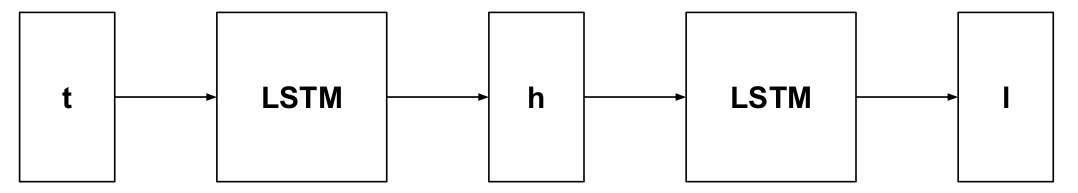
\includegraphics[scale=0.20]{Trajectory_LSTM}
\caption{Our current LSTM encoder-decoder architecture. $t$ represents a trajectory waypoint sequence, $h$ represents the embedding generated by the encoder, and $l$ is the word sequence generated by the decoder.}
\label{fig:LSTM_diagram_1}
\end{figure}

\subsection{Preprocessing}
After analyzing the Robobarista dataset, it was found  that the longest trajectory consisted of 18 waypoints. Therefore, all trajectories were fitted into tensors of 18 waypoints, with zero vectors used to pad trajectories of length less than 18. 
\par
Similarly, it was found that all phrases in the dataset consisted of less than 18 words. Accordingly, each phrase was converted into a tensor consisting of 18 one-hot vectors of dimensionality $|V|$, where $|V|$ is the size of the training set vocabulary.

\subsection{Training}

Our current architecture consists of 50 hidden units in both the encoder and decoder. We have trained our network over 1000 epochs with a batch size of 80, a mean squared error loss function, and RMSProp optimizer with a learning rate of 0.001. 

\subsection{Testing}

During testing, we feed a trajectory tensor to our network which then generates a sequence of one-hot vectors for phrases. Because every phrase in our dataset ends with a ``." token, we generate phrases of 18 tokens and prune them past the first appearance of the ``." token.  



\section{Results}


\subsection{Baseline with Point Clouds}

For the baseline, we conducted experiments using the data from each of the 5 folds, running a total of 5 trials. For each trial we created a gold reference consisting of the already known NL descriptions for each of the point clouds and a test reference consisting of the NL description returned by using the trained K-Means and KNN models.

Each point cloud in the fold test data is first inputed in the K-Means model to extract the BOF vector representation, then the BOF vector is inputed into the KNN model to retrieve the nearest neighbor of the point cloud. Lastly, we look up the NL description for the given neighbor, which is used as the output for the model. With the completed test and gold reference files we are then able to use the sentence comparison package METEOR to evaluate the accuracy of our baseline \cite{Denkowski14meteoruniversal}.

On average the baseline performed poorly, only reaching its highest performance in the first fold achieving a final METEOR score of 0.172. Figure \ref{fig:fold_1_sentence_164} shows the alignment results for two sentences from the Fold 1 test set. These results were expected as the baseline only performs a simple lookup based on nearest neighbor inference from the training set point clouds and is not able to generalize properly to the test set.

\subsection{LSTM Implementation}

Similarly to the baseline, the current LSTM architecture was evaluated using 5-fold cross validation. The results for each fold as well as the averages over all folds were computed for both the baseline and LSTM, which may be seen in figure \ref{fig:score_table}. It was found that the LSTM currently performs marginally better than the baseline, however, a Student's unpaired t-test was performed which showed that the results are not statistically significant with a p-value of 0.45. 

An illustrative example of current  LSTM performance may be seen in figure \ref{fig:lstm_alignment} (the alignment key is in figure \ref{fig:fold_1_sentence_164}). In the example, the LSTM manages to correctly infer that the trajectory pertains to pushing a button, but is unable to recognize that it is a ``white grape juice" button, something that may possibly be alleviated by the incorporation of point cloud information. Additionally, it was found that the LSTM tends to mistakenly repeat words when predicting sequences. 

\begin{figure}[h]
\centering
\begin{tabular}{|c | c | c |}
\hline
\textbf{Model} & \textbf{Baseline} & \textbf{LSTM} \\
\hline
Fold 1 & 0.172 & 0.170\\
\hline
Fold 2 & 0.141 & 0.169 \\
\hline
Fold 3 & 0.102 & 0.142 \\
\hline
Fold 4 & 0.161 & 0.139 \\
\hline
Fold 5 & 0.144 & 0.154 \\
\hline
Avg. & \textbf{0.144} & \textbf{0.155} \\
\hline
\end{tabular}
\caption{Final meteor scores for each model on each fold for 5-fold cross validation. Our current LSTM model marginally outperforms the baseline. The results are statistically insignificant with a p-value of 0.45.}
\label{fig:score_table}
\end{figure}

\section{Difficulties}\label{Difficulties}

The major difficulty we have encountered up to this point is that we have not been able yet to receive a complete trained model for the work performed by Sung et al. \cite{sung2016robobarista}. To overcome the lack of the trained model for our baseline experiments, we have decided to use Dynamic Time Warping (DTW) to compare trajectories that are associated with the point clouds. In our upcoming experiments, we will use this measure to re-rank the $k$ candidate tuples $(t,p,l)$ returned by our point cloud nearest neighbor model using their trajectories.   

Additionally, we discovered while developing our baseline experiments that the segmented points clouds for each object part are not stored in the typical Point Cloud Data (PCD) format, but instead are stored in a CSV format where each point cloud point is represented as a list of values [x,y,z,r,g,b]. To deal with this unexpected format we decided to forgo the use of NARF \cite{steder2010narf} descriptors and instead consider each point in the segmented point clouds as a key point for use in the BOF representation using the K-Nearest Neighbors method. We believe that this is a fair assumption since the point clouds were segmented in order to include only the pertinent parts of each point cloud for the given trajectories. 
\par
One final difficulty we have encountered is that the eldar GPU UTCS machines do not currently have the most current version of TensorFlow or Keras installed. Due to the size of our dataset, we have found that our current models train fairly quickly (in roughly half an hour) on our own machine's CPUs, but we have gotten in contact with Gripe in order to see if there might be some workaround allowing us to use the eldar GPU machines with our code. 


\section{Outlook}

We believe that our preliminary results show some promise for the validity of our hypothesis, although it is still ambiguous. As may be seen in figure \ref{fig:fold_1_score}, the distribution of scores for segments in the baseline seem to suggest that the model will either perform very well or very poorly on a given example. Conversely, our LSTM model's scores follows a much smoother decline in performance, which might suggest that it is more generalizable than the baseline. We hope that through the incorporation of point cloud information (as discussed in section \ref{Future Work}), the model will become more robust and may be able to surpass the baseline performance which it is currently matching.  
\par
Objectively speaking, however, comparing the current baseline and LSTM models might not be entirely fair given that they each currently operate on different input modalities (point clouds and trajectories respectively). We hope that having both our baseline and LSTM models use point cloud and trajectory information will increase performance and better elucidate the potential of our methodology. 

\section{Future Work}\label{Future Work}

In addition, to the current baseline using point clouds, we propose to conduct two more baseline experiments, one using only trajectories and the other using trajectories and point clouds. The baseline using only trajectories will only be possible to perform if we are able to receive a trained model from Sung et al. \cite{sung2016robobarista}. The baseline using point clouds and trajectories can currently be performed, however, and will be done as described in section \ref{Difficulties}. 

For the conclusion of the project, we propose to implement a two layer LSTM architecture as in \cite{Venugopalan_2015_ICCV}. Additionally, this architecture will incorporate point cloud data by concatenating the bag of feature vectors produced from a point cloud to the trajectory embedding produced by the LSTM encoding layers, the result of which will be fed to the decoder. 

Finally, we will continue to experiment with different parameters for our LSTM architecture such as through different numbers of hidden units, training epochs, and learning rates. 

\begin{figure}[h]
\centering
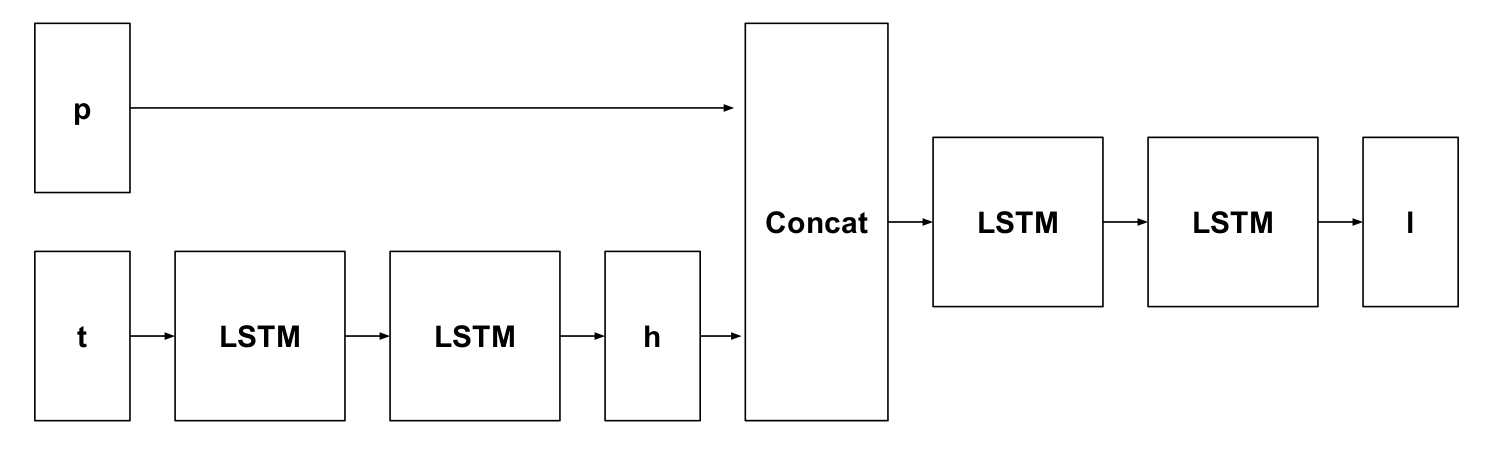
\includegraphics[scale=0.15]{Tuple_LSTM}
\caption{The proposed final architecture for our LSTM model. The network will use a double layer LSTM encoder to generate trajectory embeddings. The two layer decoder will then be trained on the concatenation between the embedding and the point cloud bag of features vector to generate word sequences.}
\end{figure}

\section{Justification of Progress}

We believe that we have made sufficient progress to put ourselves on track with the project deadlines due to the fact that we have created a full pipeline for using and evaluating our baseline and LSTM models. To continue forward we will only have to perform some slight modifications to our models to test different parameters. Additionally, the Robobarista dataset contains tools to compare trajectories using DTW, which will allow us to quickly incorporate the use of both point clouds and trajectories in our proposed additional baseline experiments. 

%\bibliographystyle{abbrv}
\bibliographystyle{IEEEtran}
\bibliography{citations}

\onecolumn

\begin{figure}[htb!]
  \centering
  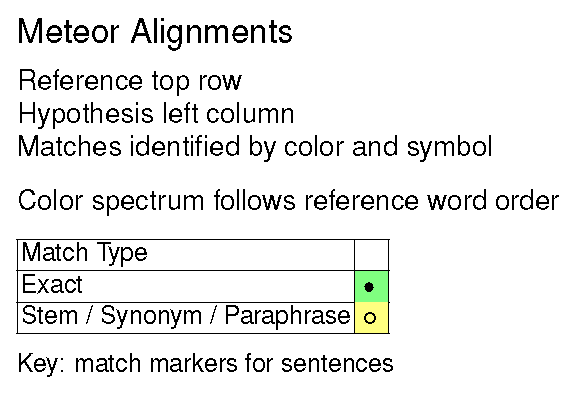
\includegraphics[width=0.25\textwidth]{meteor_alignment_key}
  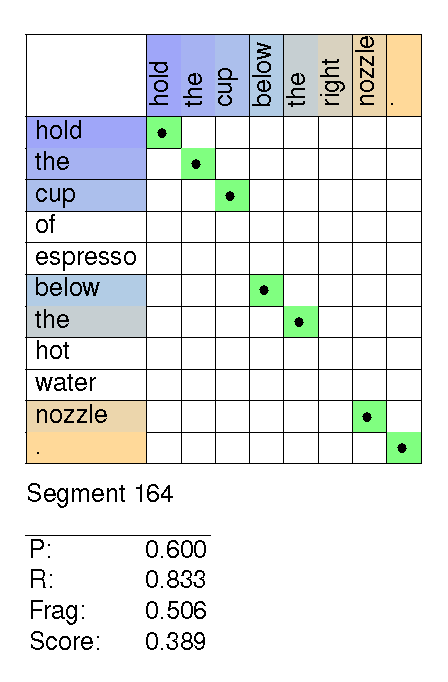
\includegraphics[width=0.25\textwidth]{fold_1_sentence_164}
  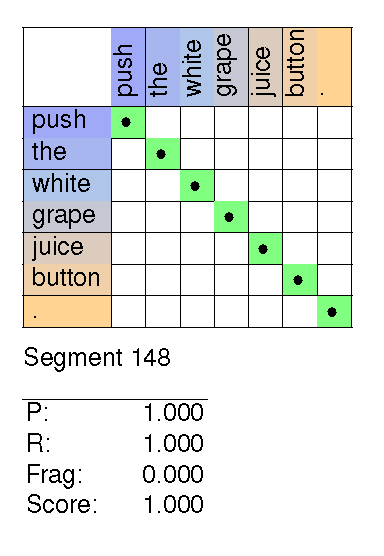
\includegraphics[width=0.25\textwidth]{fold_1_sentence_148}
  \caption{METEOR alignment for baseline fold 1 segments (i.e. phrases) 148 and 164.}
  \label{fig:fold_1_sentence_164}
\end{figure}

\begin{figure}[h]
\centering
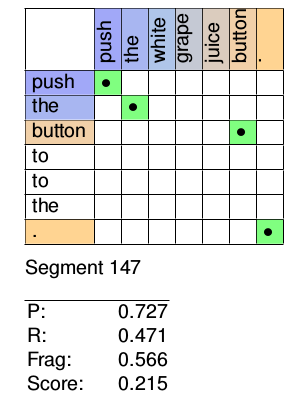
\includegraphics[scale=0.35]{lstm_alignment}
\caption{METEOR alignment for LSTM performance on fold 1 segment 147.} 
\label{fig:lstm_alignment}
\end{figure}

\begin{figure}[htb!]
  \centering
  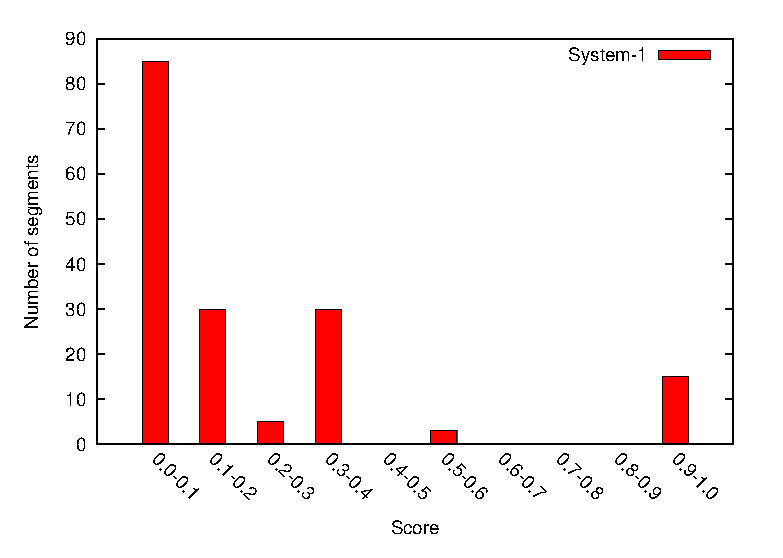
\includegraphics[width=0.45\textwidth]{fold_1_score}
  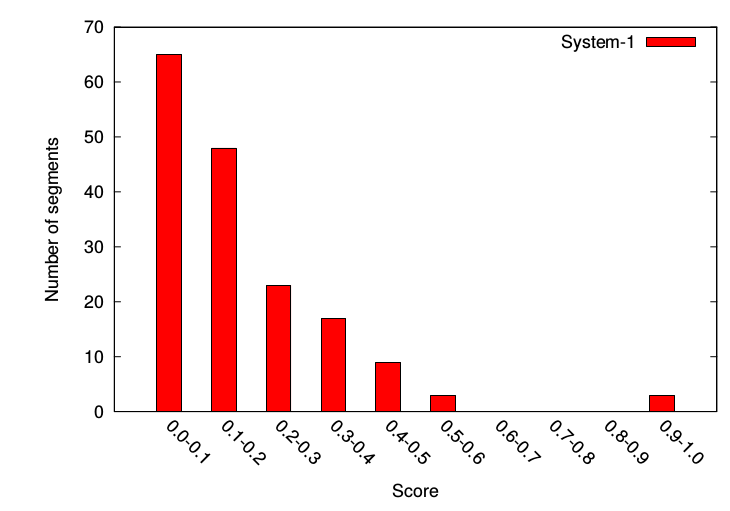
\includegraphics[width=0.45\textwidth]{lstm_fold_1_score_bar_graph}
  \caption{Segment distributions per score ranges for the baseline (left) and LSTM (right) models on the first fold of data.}
  \label{fig:fold_1_score}
\end{figure}


\end{document}
